%%% writeup.tex --- 

%% Author: bh0085@31-35-41.wireless.csail.mit.edu
%% Version: $Id: writeup.tex,v 0.0 2010/12/10 20:58:27 bh0085 Exp$


\documentclass[12pt,a4paper]{article}
\usepackage[hmargin=1in,vmargin=1in]{geometry}
\usepackage{graphicx}
\usepackage{natbib}
\usepackage{amsmath}
\usepackage{multicol}
\begin{document}

\title{Expression Prediction and Motif Discovery for the ModENCODE Fly Network}
\date{12/12/2010}
\author{Benjamin Holmes, MIT}
\maketitle
\pagebreak

\section*{Abstract} 
\noindent Target gene (TG) expression levels depend on expression levels of associated transcription factors. This project catalogs the specific interactions mapping TF level to TG level via a machine learning approach spanning clustering, regularized nonlinear regression, multitask learning, and eveventually motif discovery via a novel algorithm. Implementing predictors as supervised learners with nonlinear decision boundaries, I argue that by clustering the regulatory network for Drosophila Melanogaster (DMel) from the modENCODE consortium, it is possible to aggressively prune the set of TF interaction coefficients that arise in nonlinear learning and thus that it is possible to avoid overfitting. In order to demonstrate this, I apply models trained on time course expression data to the task of predicting differential gene expression across four DMel cell lines. Whereas the question of discovering regulatory motifs is latent in the learning algorithms of the first sections, I conclude this project by presenting an algorithm with which to explicitly compute motifs via a stochastic search.

\begin{multicols}{2}


\section{Background}


Serving as a reservoir of heriditary information passed from ancestor to child for billions of year, genomic DNA has enabled and recorded the history of life as it is known on the planet earth. For its stability and simplicitly, it is apparently sufficient to serve as a universal encoding of the requisite information to build life as we know it. For the same reasons, the genome - viewed as a one dimensional sequence of characters drawn from a quaternary alphabet - is a woefully incomplete description of living systems in their full range of dynamics and diversity.


These dynamic interactions between constituents of bilogical systems are best understood in terms of interconnected networks organizing biological elements. Manifested as protein protein physical interactions in the cell, inter and intra-tissue signalling cascade spanning or electrical control systems spanning entire organisms, biological networks are responsible for the dynamics of life.

Among these, the regulatory network characterized by a directed set of interaction edges between coding genes and their protein products possesses special significance. In multicellular orgranisms, regulatory networks are known to coordinate a broad range of interactions across a range of time and spatial domains - whether in governing heat shock response in bacteria or dictating the differentiation of stem cells into an embryonic limb - and in the era of high throughput biochemistry, the resolution and scope of our knowledge of regulation is increasing at an accelerating pace.

Meanwhile on geologic timescales, evolution of regulatory interactions represent the bulk of the evolutionary difference between allied and distantly related species. Thus, in the development of higher animals from single celled eukaryotes, increasing tissue specialization, lifestyle and ecosystem change, and the development of intelligence have been accompanied by increasing density of regulatory edges more reliably than increasing genomic size.

Accordingly, a sophisticated understanding of human physiology in theory or for practical purposes such as the treatment of disease must include a sophisticated understanding of the human regulatory network. In consideration of the fact that much of our knowledge of human systems comes from experimentation on closely allied species, it is necessary not only to understand the lone regulatory network of the human body but to have a methodology with which to extrapolate network inference between species. Recalling that regulatory systems are recepticles of the builk of evolutionary change, it is clear that robust identification of network motifs and interactions over philogentic trees is no small task. High throughput approaches are required and machine learning approaches are implicated.

Accordingly, this project will analyze a specific network: the regulatory network developed for the fly D. Melangoster by the large scale experimental and bioinformatic consortium modENCODE in search predictive relationships between TFs and repeated regulatory motifs. In the modENCODE project\cite{RefWorks:30}, independent data sets such as DNA-protein binding, de novo motif discovery, and coexpression datasets were compiled to produce a network cataloging the complete set of regulatory interactions between protein transcription factors (TFs) and target genes (TGs) by supervised and unsupervised methods with largely (but not completely) concurrent results. This project will use the unsupervised network and expression data covering 8316 TGs an 541 TFs to attempt expression level prediction of TGs from network-associated TFs.

Neither formulation of the prediction problem or the idea of attacking it with machine learning approaches is new. Using the same data set as in this paper, modENCODE\cite{RefWorks:30} for example uses regularized linear regression to derive interaction coefficients corresponding to real numbered edge weights in the DMel unsupervised network that solve the regression problem. While this method is easily automated to predict the interaction of large numbers of genes and TFs, the individulal weights learned by the the interaction may not reliably imply biological interaction.

Others such as Segal\cite{RefWorks:26} have taken a biophysical approach. Applying thermodynamic models in order to predict transcription factor residency, Segal models the regulation of a smaller number of genes important to the development of segmentation of drosophila as the product of competitive interactions between large numbers of weakly bound TFs. In the Segal approach, the model learned immediately implies a physical mechanism but its predictive success leans heavily on weak binding and interactions between TFs. In so far as this may be an accurate model of underlying biology, we should not expect an accurate model to behave otherwise. We suspect however that to train a model to predict both TF occupancy, TF-TF interactions and TF-gene inhibition/enhancement requires manipulating a dangerously large parameter space and may induce overfitting. We may find our suspicion confirmed by the tendency of Segals model to place much of the burden of regulation on weak - thus abundant - TF-gene interactions.

In any case, the current state of the art applies machine learning methods to predict expression of single genes from associated TFs. These methods take as input one gene and an assumed network, producing as output a model for its expression. Augmented by interpolation methods and cluster-baseline predictions, the state of the art can do a fairly good job of predicting expression but may overfit the data to the extent that individual TF-gene predictions may be unreliable. It suggests no reliable means of decoding TF-TF interactions and confronted by a massive network with many genes presumably regulated in similar fashion, it learns gene by gene in the manner of single-task learning.

In this paper I will implement regression models that predict TG expression from TF levels in a nonlinear decision space by considering high dimensional feature vectors constituted by interaction terms combining products of TFs up to degree $d$. In the first section of results, I suggest that by clustering the network from modENCODE, it is possible to break the space of TFs and TGs into associated subsets between which the prediction problem can be approximated independently. 

One purpose of breaking the prediction problem up like this is to reduce the number of nonlinear interaction terms forming feature vectors. In the second results section, I implement multitask learning and explicit feature selection by reducing mutual information to advance towards the same goal: by aggressively reducing the parameter space of the learning problem, I claim that it is possible to minimize overfitting to increase accuracy and motif signifiance. Finally, I implement a novel prediction method hybridizing a genetic algorithm (GA) for high bandwidth parallelizable search with neural network based gradient descent for evaluating predictability of GA-derived interaction topologies. I suggest that with my algorithm, it will be possible to discover regulatory motifs quickly and easily.



\section{Results \& Discussion}
\subsection{Clustering}\label{clustering}
The network, covering $n_g \sim 8316$ target genes and $n_f = 541$ transcription factors was available to me in the form of an $n_g\times n_f$ adjacency matrix $A$ giving gene edges that I thresholded on the advice of its creator to treat as binary array having $217,426$ edges corresponding to likely regulatory interactions. Expression data was available to me as mRNA levels for genes and factors at 30 time points during DMel development and seperately for 4 different cell lines.

In order to normalize expression levels, perform multitask learning and establish a search space for feature selection in the nonlinear learning problem it was first necessary to break the data set into clusters associating subsets of DMel TFs and TGs. By clustering the network into similarly sized clusters associating on the order of $10-100$ genes to a similar if slightly smaller number of TFs, I planned ot reduce the $\sim 8000$ gene learning problem into $\sim 800$ similar subproblems. 

Network topology suggested that TFs would be reused between clusters more than TGs. With this in mind and because standard clustering algorithms such as $k$-means are best at forming exclusing clusters. I proceeded by clustering TGs into groups and then associating them with shared TFs.

Desiring a more expressive clustering matrix than the binary network adjacency matrix $A$, I experimented with several similarity matrices upon which to do row clustering to group TFs.

\begin{eqnarray*}
S_{ij}^{N} &=& \text{jaccard index\footnotemark \hspace{1ex}TG$_i$, TG$_j$}\\
S_{ij}^{int}&=& \text{int. dist.\footnotemark \hspace{1ex}from TG$_i$, TG$_j$}\\
S^{\text{SVD}} &=& U | A = U\Sigma V^T, U,V \text{ unitary}
\end{eqnarray*}
\addtocounter{footnote}{-2}
\stepcounter{footnote}\footnotetext{For TG$_i$, TG$_j$, the jaccard index, $\mathcal{J}_{ij}$, is the size of the intersection of the sets of their respective TFs over the size of their union. Later as an ad hoc heuristic, I will use a weighted jaccard index computing the same quantity but dividing the contribution from each TF by its out degree in the network in order to place special weight on highly specific TF-TG interactions in clustering TGs.}
\stepcounter{footnote}\footnotetext{I define interaction distance by the minimum number of steps to go from one TG$_i$ to TG$_j$ by row and columnwise traversal of nonzero elemnents of the adjacency matrix $A$. Equivalently:
\begin{equation} S^{\text{int}}_{ij} \equiv \min_{k > 0} \left\{ k | \left( \left( A^k \right) _{ij} > 0 \right) \right\}\end{equation} }

Hoping to find $~100$ gene cluster of moderate size, I ran both $k$-means with $k=100$ and hierachical clustering halted at the $n_c = 100$.

Clustering produced clusters of very different sizes - presumably as a result of the hierarchical distribution of DMel TFs in the nearly scale free network. In order to even out cluster sizes, I could have manually rerun the clustering algorithm to split up large clusters but a less ad hoc approach was to weight elements of the similarity matrix to reduce the impact of hub TFs regulating large numbers of TGs. Doing this and rerunning the clustering reduced cluster size discrepencies somewhat.

In order to even out cluster sizes more and to process the data more transparently, I chose to form clusters grouping TG siblings. By choosing a jaccard index fixing a minimum fraction of parents that two TGs would have to share in order to be considered siblings, I defined a (possibly singleton) sibling cluster centered on each TF. By this method, I was able to find gene clusters of manageable size to which I could easily associate a set of mostly shared transcritiption factors. Fig.\ref{fig:clusters} pictures clusters derived from this and other methods. 

By distinguishing between factors shared by all or most of a cluster and those shared by only one or a few TGs, I was given a ready criterion with which to discard network edges during feature selection and a natural grouping of TFs into shared and unshared inputs in the neural net formulation of the prediction problem outlined in \ref{selection} and diagrammed in fig.\ref{fig:gagd}. 

\begin{figure*}[h]
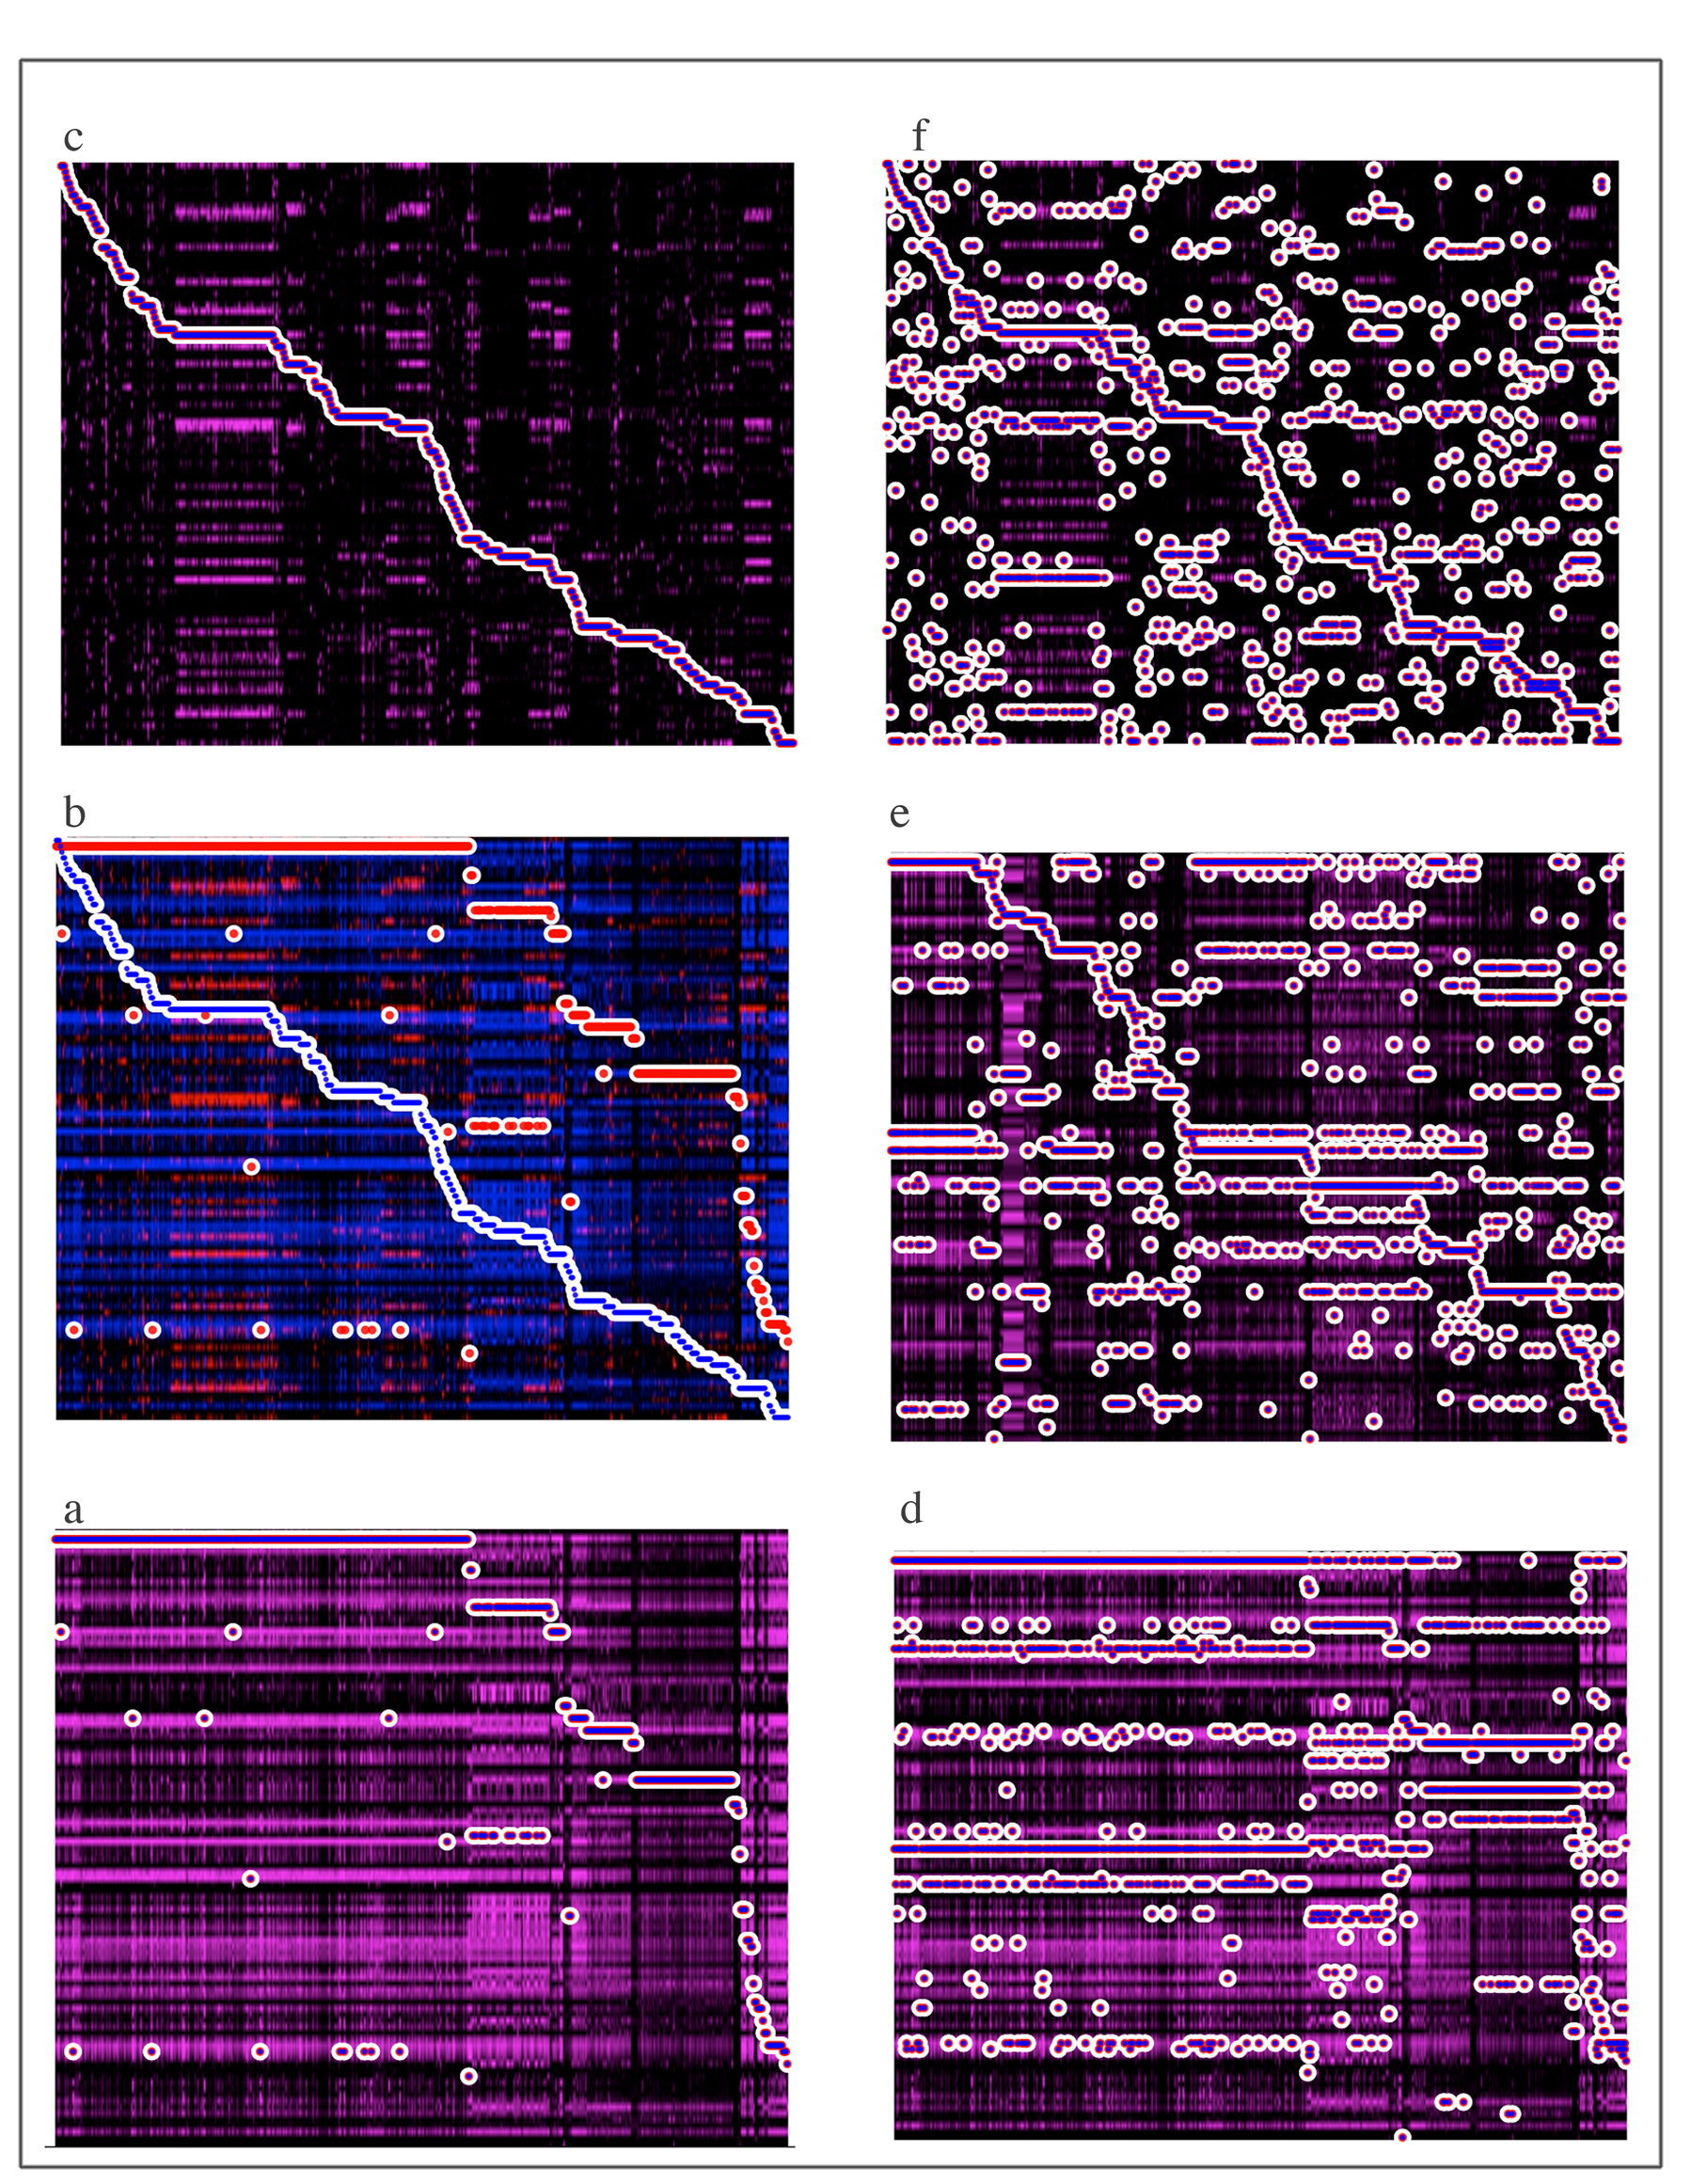
\includegraphics[width = 6in]{figs/clusters.pdf}
\caption{Clusters derived by three different methods in two different views. In each image, TFs appear on the X axis and clusters are indexed on the Y axis. Image brightness indicates the frequency with which a TF,x regulates the genes in the cluster,y. For each TF, the cluster within which it participates most strongly (a-c) and the three clusters within which it participates most strongly (d-f) are marked with dots. 
Figures a,b,c plot the centers of clusters derived by k-means using $S^{\text{jac}}$ (a) and jaccard clustering (c) with normalized TF weighting. Plot (b) overlays the two clusterings in red and blue in order to demonstrate the relatively more even distribution of clusters across TF space in the normalized weighting scheme. Figs d,e,f plot the top 3 clusters regulated by $S^{\text{jac}}$, $S^{\text{svd}}$, and normalized jaccard respectively. Normalized jaccard has a distribution of cluster sizes to the final sibling based clustering once cluster duplicates are removed.}
\label{fig:clusters}
\end{figure*} 

\subsection{Multitask Learning and Feature Selection}\label{FS}

For clusters associating a set of transcription factors $\mathcal{F}$ with a set of target genes $\mathcal{G}$ having sizes $n_f$, $n_g$, the time series data set that I will use for training contain $30*(n_f + n_g)$ expression level datapoints $E_f$, $E_g$. A standard linear model predicting elements of $\mathcal{G}$ individually via $n_f$ weights from $E_f$ would have $n_f\times n_g$ paramaeters and so for even moderately sized clusters such as those found in \ref{clustering}, the linear prediction may be incompletely or barely specified and may lack sufficient expressiveness to distinguish biological results from biological or eperimental noice. Nonlinear learning methods which we will explore suffer from the same problem even more severely: a second degree model running linear regression using features corresponding to pairwise products $f_i \times f_j, f_{i,j} \in \mathcal{F}$ will have on order $n_f^2\times n_g$ parameters\footnote{order $n_f^d \times n_g$ for degree $d>1$} and the same regression problem would be unspecified for clusters as small as $n_g=n_f=7$ and barely specified even for smaller ones.

These observations imply that feature selection is in order if overfitting of the available data is to be avoided. In this project, I have taken two approaches to feature selection once clusters have been determined as in \ref{clustering}: they fall into the general classes of feature selection via multitask learning and via exclusion of features with high mutual information content.

In the multitask feature selection task such as multisvm\cite{RefWorks:28}, parameters are shared between between some or all genes in a cluster to reduce the parameter space to the order of $n_f^d\times (O(1))$ for a regression with order $d$ interactions. In mutual information minimizing approaches such as \textit{MRNET}\cite{RefWorks:29}, covarying features - thus, TF interaction terms that do not represent independent features - are removed from the dataset or merged. By removing all but $k$ interaction terms, it is thus possible to reduce the parameter count for the clustering problem to order $k\times n_g$ setting $k$ as desired to choose regularization agressiveness.

I have implemented the multitask ``all parameters shared regularization'' and feature selection via merging covarying factors for feature vectors with interactions $d \in \{1,2 \}$ and solved the regression problem using regression trees (at the suggestion of Sushmita Roy) and random forests of binary decision trees to differentiate between above mean and below mean expression levels. By subtracting mean cluster expression levels and dividing by cluster standard deviation for $E_{f,g}$ to yield uncorrelated expression z-scores at each time point, it was possible to more accurately describe feature dependence and implement slightly sophisticated interaction pruning.

Over a set of 20 similar clusters regulated by different TFs, average mean squared errors (Zscore) in generalization from time series to cell line datasets were 4.87 / 5.67  / 7.45 for normalization+feature selection, tree regression with cluster based feature selection, and tree regression trained on random TFs respectively. In fig.\ref{fig:reg} I demonstrate the processing pipeline with cluster-based (but not mutual information-based) feature selection and zscore decorrelation. In fig.\ref{fig:sample}, I show time series predictions and cell line generalization for a sample gene via few different methods. 

I note but do not show a plot to demonstrate, that regularization and multitask learning do not improve accuracy over the  training set but that on average they improve prediction generalization error, implying that they are in fact minimizing data overfit.

\begin{figure*}[h]
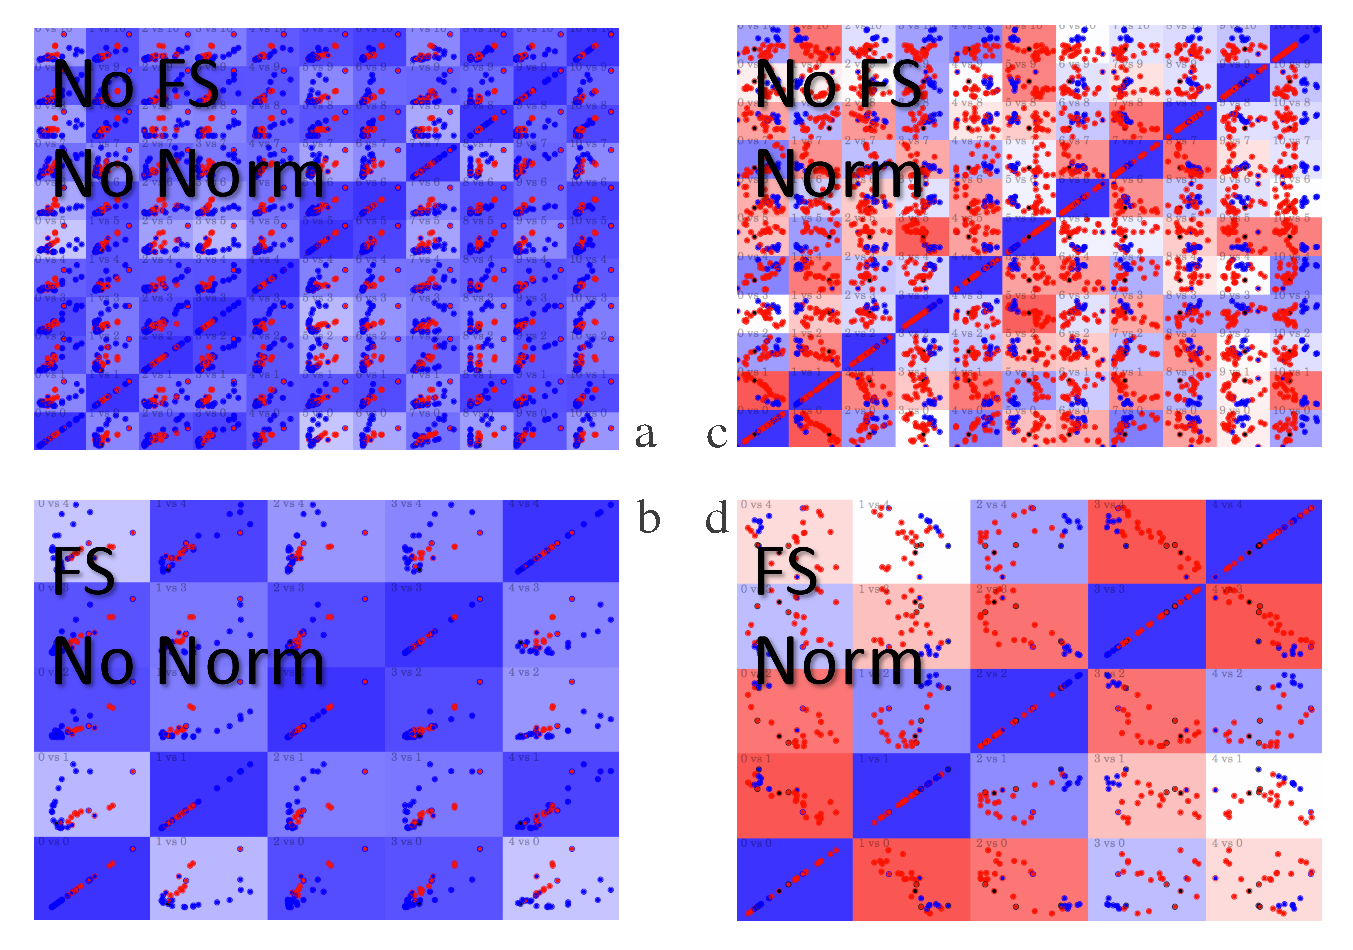
\includegraphics[width = 6in]{figs/regularization}
\caption{The regularization pipeline. Each cell in each subfigure expression levels for a fixed TG as on/off (blue/red) with dot locations determined by expression levels of a pair of TFs corresponding to the X and Y axis. The coloring of the $i,j^{th}$ cell indicates the covariance of expression of the $i$ and $j^{th}$ tfs associated with the TG. Uncorrelated TFs $i,j$ - thus, those with low mututal information - appear as nearly white cells while (anti-)correlated TFs appear as (red) blue cells. Feature selection in subfigures with ``FS'' indicated is selection for cluster-shared TFs and ``Norm'' indicates that features have been transformed to maximize independent information by the Zscoring method outlined in \ref{FS} }
\label{fig:reg}
\end{figure*} 


\begin{figure*}[h]
\includegraphics[width = 6in]{figs/prediction}
\caption{Prediction for time series and generalization to cell line for normalized/feature selected and non-normalized/non-feature selected expression. ``Unclustered'' indicates the naive prediction task using all of the TFs for the gene predicted by the network. In the example shown, this approach fails to generalize from training on time series to cell line. The figure on the lower left is a reminder that even randomly selected TF subsets will make correct predictions some of the time.}
\label{fig:sample}
\end{figure*} 

\subsection{Motif Discovery}\label{selection}

The final goal of this project was to explore techniques for regulatory motif discovery. Several of the methods implemented including regression of degree $d$, decision trees, and regression trees incorporate feature interaction in predicting expression levels. To the extent that these models not only correct predictly but also bear internal similarity to biological mechanisms, they are suggestive of regulatory motifs. Supposing however, that meaningful motifs may have been excluded by feature selection and multitask learning designed to build generalizable learners in \textbf{\ref{FS}}, this project seeks to enumerate regulatory motifs explicitly via a novel novel method.

To this end, I have designed a hybrid algorithm meshing a genetic algorithm (GA) with gradient descent (GAGD) for which GA ``genomes'' each specify a set of connections in a neural network for predicting gene expression levels.

In particular, each neural network in the population of the genetic algorithm  consists of a common set of nodes: an input layer $\mathcal{I}$ having one node per $f \in \mathcal{F}$, a linear output layer $\mathcal{O}$ having one node per $g \in \mathcal{G}$ and a hidden layer with sigmoidal activation containing a set of nodes $\mathcal{H}_g$ each connecting exactly one element of $\mathcal{O}$ to a subset of $\mathcal{I}$ plus a set $\mathcal{H}_c$ each connecting a subset of $\mathcal{O}$ to a subset of $\mathcal{I}$. 

When the network is activated, a signal flows from $\mathcal{I}$ through available weighted connections to $\mathcal{H}_g$, $\mathcal{H}_c$ whose output is a sigmoid\footnote{sigmoidal activation is a smoothed generalization of the perceptron (on/off) activation rule} of the weighed sum of inputs which is weighted and passed on to available connections to $\mathcal{O}$ and used for prediction. $h \in \mathcal{H}_c$ can be thought of as computing shared regulatory motifs biasing expression for part or all of the gene cluster while $h \in \mathcal{H}_g$ can be thought of computing gene specific regulatory motifs. The scheme of possible connections in GAGD is outlined for a small cluster in fig.\ref{fig:gagd}

\begin{figure*}[h]
\includegraphics[width = 4in]{figs/gagd_schematic}
\caption{The full set of allowed connections in a network for a cluster with $n_g = 2$, $n_f = 8$, or the case where two TFs are shared by g0 and g1 and the rest are associated with either g1 or g0 with no direct connections permitted between shared TFs and gene hidden units. Nets generated  by GAGD will only realize a subset of these connections.}
\label{fig:gagd}
\end{figure*} 

Learning GAGD is broken into two parts:
\begin{description}
\item[GA]{In the genetic learning, a random set of network topologies  is drawn up and encoded into a population of genomes specifying a subset of the allowed upon which signals are allowed to flow and starting network weights $w_{ij} \in {-1,0,1}$. The fitness function will be computed by the success of training in the GD learning phase at which point, genomes are selected to undergo mutation and crossover to build a new generation by tournament selection\footnote{In tournament selection, pairs of genomes from the population are selected at random, intra-pair fitness values are compared and the higher fitness of the pair is allowed to move to the next generation. Tournament selection maintains population diversity more reliably than simpler methods such as fitness proportional selection.}}
\item[GD]{In order to evaluate the fitness function of each neural-net encoded by genomes in the population, the network is initialized with starting weights specified by the genome and allowed to train for a small number of iterations through the training data. Weights for allowed edges are modified by rapidprop \footnote{RapidProp is a fast training modification of the standard gradient descent based learning algorithm backprop. It is useful here because it rapidly searches the weight space of an encoded network for locally optimal solutions, allowing quick characterization of the local optimality of the genome-encoded network} and the fitness score returned by gradient descent is proportional to the fraction of training points correctly predicted to within some prespecified threshold for all genes.\footnote{the ``fraction correct'' metric is more useful here than say - mean squared error - because (1) it yields a strictly positive fitness function and (2) because training is not being allowed to run sufficiently long for a tight fit to data to be achieved. For the purpose of rapid topology evaluation, direct minimization of MSE is unnecessary.}} 
\end{description}

\begin{figure*}[h]
\includegraphics[width = 5in]{figs/GA_pop}
\caption{Four genome-encoded neural networks drawn from a random population before and after a single round of training. Allowed connections are blue, red or white representing net connection weights of $+1,-1,0$ respectively; edge opacities are proportional to the magnitude of edge weight. After a round of training, allowed edges initially having zero weight choose a sign and fade in; edges forbidden by net topology remain zero.}
\label{fig:gapop}
\end{figure*}

Fig.\ref{fig:gapop} show an example subset of a randomly NN generated population at initializatiokn and immediately after. In order to encourage stochastic exploration of the space of network topologies and discourage commitment of the GA population to local optima, each generation of nets is trained and evaluated over a randomly chosen subset of all training examples. While the algorithm and genomic representation are in place, some details of the implementation still await completion and topology search and motif categorization remain objects of future work.

\section{Future Goals}
Several goals remain outstanding in each of the three sections of this project.
\begin{description}
\item[Clustering:]{the clustering method chosen\footnote{1: For each TG, associate siblings at some weighted jaccard index --see footnote above--$(.7)$ giving a minimal fraction of TF sharing. 2: To each of $N_g$ derived clusters associate a set of TFs shared by a specified fraction $(.7)$ of TGs and $|\mathcal{G}|$ sets of unshared TFs. 3: Filter out any clusters having more than $75\%$ genes in common.} is a useful heuristic in so far as it produces a large number of similarly sized clusters but as it relies on an arbitrarily chosen set of parameters, future attempts will either have to compare prediction quality across different clustering parameters or switch to a principled method. Further, since TFs controlling large numbers of TGs are assigned reduced weights in the current clustering schema, cluster assignment could be better motivated if this normalization was theoretically justified or accomplished in a more principled manner\footnote{Such a ``more principled'' manner would perhaps take the network's hierarchy into account and differentiate hub TFs from non-hubs in their influence over clustering. Fundamentally, any such approach will have to deal with the fact that in an approximately scale free network, it is unreasonable to expect to generate clusters of a constant size and handle adapt downstream learning accordingly.}}
\item[Feature Selection:]{Selection via mutual information currently only looks at expression covariance as manifested in zscore computed from $\mathcal{F},\mathcal{G}$ mean expression and standard deviation. More general methods for determining mutual information exist (e.g MRNET\cite{RefWorks:29}) and they would probably benefit our model. Moreover, by taking only the simplified ``shared parametrization for all $\mathcal{G}$'', I am missing important cases where TGs regulated uniquely or a subset of cluster TGs are regulated by some motif. The analysis shown demonstrates only that via multitask learning it is possible to some extent to trade expressiveness for generalization accuracy. A more advanced algorithm would probably implement partial feature pooling (as in multisvm \cite{RefWorks:28}).}
\item[Motif Discovery:]{ Results from feature discovery still await a final implementation. Since the GA fitness evaluation is a naturally parallel task, an interesting and relatively straightforward part of this implementation will be spreading evaluation (ie: NN RapidProp) across multiple processors. I strongly suspect that with proper tweaking, GAGD will be a fertile platform for motif discovery and furthermore that genetic operations such as crossover will be useful tools for discovering motifs regulating a subset of the data and extending them to others. To this point, the current genomic representation of a neural network topology could presumably be optimized to encourage this kind of exchange\footnote{In its current form, the GA encodes NN topologies as grouped triplets specifying connection nodes and weights: 
\begin{align*} 
\text{Genome} =...&[N_{\text{cxns from $\mathcal{I}_{\text{shared}}$ to $\mathcal{H}_c$}}][(i_0,h_0,w_0),(i_1,h_1,w_1)...(i_{N_{\text{cxns}}},h_{N_{\text{cxns}}},w_{N_{\text{cxns}}})]\\
&[N_{\text{cxns from g1 TFs to $\mathcal{H}_1$}}][(i_0...)]...
\end{align*}
}. }
\end{description}


Because much of the work of this project has been motivated by concerns of model overfitting, especially when training models having coupled feature vectors, the emphasis of future work will probably shift as more data becomes available. Although this different emphases would have been advised if -say: an order of magnitude more data was available- the basic approach of clustering and testing different methods of model regularization would remain fundamentally sound. Because uncovering regulatory motifs of biological relevance is a goal in its own right, an approach that simply predicts or generalizes well is not fully satisfactory if it does not suggest motifs. Rather: as more expression data becomes available, cluster-wide prediction mindful of the network hierarchy will be useful in pruning the network itself of indirect links and suggesting new network edges. One interesting test will be to see whether new links suggested by GAGD correspond to disagreements between the unsupervised network that has been the basis for the work in this paper and the supervised network that exists in similar form but was not used. 


\section{Proposal Comparison}

The original proposal for this project ran along the same conceptual lines as the final version: in order to improve on previous work predicting DMel gene expression from modENCODE data I intended to implement nonlinear models from which it would be possible to deduce not only individual prediction weights giving gene expression levels as a function of associated transcription factors but interaction terms suggesting conditional dependence of TFs upon one another. It was clear from the start that aggressive reduction of parameter space would be in order and that multitask learning could be helpful.

What was not completed was specification of a subset of regulatory motifs presumed with high probablility to be controlling inter and intra cluster expression of target genes. Suspecting that stringent feature selection and normalization in \ref{FS} has caused relevant motifs and motif constituents to be discarded, I have not attempted to read a list of motifs from nonlinear interaction terms with high weights in \ref{FS}. While GAGD in \ref{selection} explicitly attempts feature selection and is exactly the approach that I outlined in my project proposal, results from it are not yet available; thus, the goals set out in my proposal are not yet complete.

\section{My Experience}

The most fun part of the project for me was mapping out the hybrid algorithm that I have presented for meshing genetic search with a gradient descent optimization problem. If I was to restart this project from the beginning, I could have spent the entire time characterizing its activity and I suspect that turning it into a reliable method for regulatory motif discovery could have filled the bulk of this paper given sufficient room and time.

I also would like to have incorporated more biological context into the results section of this paper. I suspect however that at this point enough of the hard word is done and sufficient formalism has been developed to allow a fairly straightforward attack on for example gene clusterings built by tissue specific expression. 

Overall, getting data into a workable form took more time than I had expected and necessitated construction of a toolset for caching data sets into my computer's memory without which the project would have ground to a halt.

\section{Peer Reviews} 

I enjoyed the peer review process immensely. One useful part was being asked to defend my choice of a Neural Net as a prediction model during the verbal peer review session. Forced to defend my choice or reconsider in light of the fact that NN training is slow and prone to stall in local optima, I realized that local optima were exactly what I was looking for in regulatory motif discovery. 

In particular, because my goal was to test the predictive capacity of a motif corresponding to perturbations about a topology generated by a genetic algorithm, I was not looking for a learning with a tendency to globally converge. By seeding nets not only with topologies but weights, I was able to shift even more of the training burden off of the neural net and to focus it on the task of local maximization of the fitness function. Because local optima are quickly reached by the RapidProp training algorithm, I was able to dramatically reduce iterations and thus fitness function evaluation time, thereby allowing an increase in GA population size and an improvement in topology search bandwidth.

\section{Division of Labor}

The initial plan for the project was for me to write the bulk of the learning algorithms for feature selection, multitask learning, and motif discovery while my partner would study the structure of the network and expression data in order to design a principled, non-exclusive clustering algorithm yielding sets of genes and regulating factors backed up by multiple lines of evidence. Given such a clustering, we planned to put our results in biological context, enumerating regulatory motifs in particular tissues, perhaps at different stages of development. A family emergency came up and my partner had to leave the country. I think that he was under a lot of stress before leaving because to date, all of the work on this project has been my own.




%%%%##########################################################################


\bibliographystyle{nature}
\bibliography{refs}


\end{multicols}  
\end{document}
 